Il periodo di Progettazione architetturale ha inizio con la presentazione della RR e finisce con la consegna della RP.\newline
In questo periodo, le attività svolte sono le seguenti:
\begin{itemize}
	\item \textbf{Incremento:} modifiche incrementali ai seguenti documenti, secondo la valutazione della Revisione dei Requisiti:
	\begin{itemize}
		\item Analisi dei requisiti;
		\item Piano di progetto;
		\item Piano di qualifica;
		\item Glossario;
		\item Norme di progetto.
	\end{itemize}
	\item \textbf{Technology baseline:} attività che consta nell'individuare tutte le librerie, framework, pattern e linguaggi di programmazione necessarie per realizzare il prodotto software. I componenti del gruppo prenderanno dimestichezza con tali tecnologie realizzando il Proof of Concept, che nel caso del gruppo \textit{SWEight} consiste nel realizzare alcuni componenti che verranno impiegati all'interno del prodotto software. L'attività è soggetta a verifica {Agile}\ped{G} e il suo esito è bloccante, pertanto la sua priorità è elevata. 
\end{itemize}
I documenti con priorità maggiore sono: Norme di Progetto, il cui contenuto è necessario definire la {way-of-working}\ped{G} per realizzare il {Proof of Concept}\ped{G}, e Analisi dei Requisiti, per delineare più precisamente i requisiti descritti nel periodo di investimento.
\begin{figure}[H]
	\begin{center}
		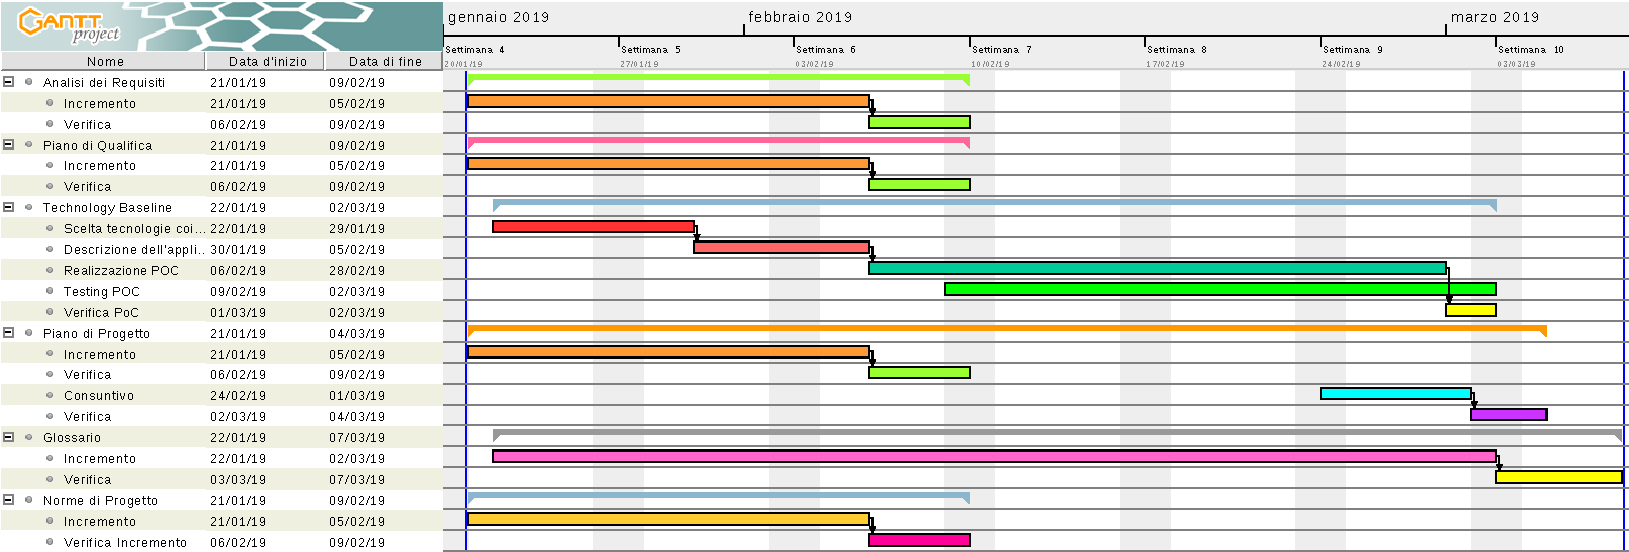
\includegraphics[width=17cm,height=\textheight,keepaspectratio]{Pianificazione/Progettazione.pdf}
	\caption{Diagramma di Gantt del periodo di Progettazione architetturale}
	\end{center}
\end{figure}